\documentclass[ignorenonframetext,]{beamer}
\setbeamertemplate{caption}[numbered]
\setbeamertemplate{caption label separator}{: }
\setbeamercolor{caption name}{fg=normal text.fg}
\beamertemplatenavigationsymbolsempty
\usepackage{lmodern}
\usepackage{amssymb,amsmath}
\usepackage{ifxetex,ifluatex}
\usepackage{fixltx2e} % provides \textsubscript
\ifnum 0\ifxetex 1\fi\ifluatex 1\fi=0 % if pdftex
  \usepackage[T1]{fontenc}
  \usepackage[utf8]{inputenc}
\else % if luatex or xelatex
  \ifxetex
    \usepackage{mathspec}
  \else
    \usepackage{fontspec}
  \fi
  \defaultfontfeatures{Ligatures=TeX,Scale=MatchLowercase}
\fi
% use upquote if available, for straight quotes in verbatim environments
\IfFileExists{upquote.sty}{\usepackage{upquote}}{}
% use microtype if available
\IfFileExists{microtype.sty}{%
\usepackage{microtype}
\UseMicrotypeSet[protrusion]{basicmath} % disable protrusion for tt fonts
}{}
\newif\ifbibliography
\hypersetup{
            pdftitle={242 Final Project},
            pdfauthor={Lizzy Kinnard and Shelley Facente},
            pdfborder={0 0 0},
            breaklinks=true}
\urlstyle{same}  % don't use monospace font for urls
\usepackage{color}
\usepackage{fancyvrb}
\newcommand{\VerbBar}{|}
\newcommand{\VERB}{\Verb[commandchars=\\\{\}]}
\DefineVerbatimEnvironment{Highlighting}{Verbatim}{commandchars=\\\{\}}
% Add ',fontsize=\small' for more characters per line
\usepackage{framed}
\definecolor{shadecolor}{RGB}{248,248,248}
\newenvironment{Shaded}{\begin{snugshade}}{\end{snugshade}}
\newcommand{\KeywordTok}[1]{\textcolor[rgb]{0.13,0.29,0.53}{\textbf{#1}}}
\newcommand{\DataTypeTok}[1]{\textcolor[rgb]{0.13,0.29,0.53}{#1}}
\newcommand{\DecValTok}[1]{\textcolor[rgb]{0.00,0.00,0.81}{#1}}
\newcommand{\BaseNTok}[1]{\textcolor[rgb]{0.00,0.00,0.81}{#1}}
\newcommand{\FloatTok}[1]{\textcolor[rgb]{0.00,0.00,0.81}{#1}}
\newcommand{\ConstantTok}[1]{\textcolor[rgb]{0.00,0.00,0.00}{#1}}
\newcommand{\CharTok}[1]{\textcolor[rgb]{0.31,0.60,0.02}{#1}}
\newcommand{\SpecialCharTok}[1]{\textcolor[rgb]{0.00,0.00,0.00}{#1}}
\newcommand{\StringTok}[1]{\textcolor[rgb]{0.31,0.60,0.02}{#1}}
\newcommand{\VerbatimStringTok}[1]{\textcolor[rgb]{0.31,0.60,0.02}{#1}}
\newcommand{\SpecialStringTok}[1]{\textcolor[rgb]{0.31,0.60,0.02}{#1}}
\newcommand{\ImportTok}[1]{#1}
\newcommand{\CommentTok}[1]{\textcolor[rgb]{0.56,0.35,0.01}{\textit{#1}}}
\newcommand{\DocumentationTok}[1]{\textcolor[rgb]{0.56,0.35,0.01}{\textbf{\textit{#1}}}}
\newcommand{\AnnotationTok}[1]{\textcolor[rgb]{0.56,0.35,0.01}{\textbf{\textit{#1}}}}
\newcommand{\CommentVarTok}[1]{\textcolor[rgb]{0.56,0.35,0.01}{\textbf{\textit{#1}}}}
\newcommand{\OtherTok}[1]{\textcolor[rgb]{0.56,0.35,0.01}{#1}}
\newcommand{\FunctionTok}[1]{\textcolor[rgb]{0.00,0.00,0.00}{#1}}
\newcommand{\VariableTok}[1]{\textcolor[rgb]{0.00,0.00,0.00}{#1}}
\newcommand{\ControlFlowTok}[1]{\textcolor[rgb]{0.13,0.29,0.53}{\textbf{#1}}}
\newcommand{\OperatorTok}[1]{\textcolor[rgb]{0.81,0.36,0.00}{\textbf{#1}}}
\newcommand{\BuiltInTok}[1]{#1}
\newcommand{\ExtensionTok}[1]{#1}
\newcommand{\PreprocessorTok}[1]{\textcolor[rgb]{0.56,0.35,0.01}{\textit{#1}}}
\newcommand{\AttributeTok}[1]{\textcolor[rgb]{0.77,0.63,0.00}{#1}}
\newcommand{\RegionMarkerTok}[1]{#1}
\newcommand{\InformationTok}[1]{\textcolor[rgb]{0.56,0.35,0.01}{\textbf{\textit{#1}}}}
\newcommand{\WarningTok}[1]{\textcolor[rgb]{0.56,0.35,0.01}{\textbf{\textit{#1}}}}
\newcommand{\AlertTok}[1]{\textcolor[rgb]{0.94,0.16,0.16}{#1}}
\newcommand{\ErrorTok}[1]{\textcolor[rgb]{0.64,0.00,0.00}{\textbf{#1}}}
\newcommand{\NormalTok}[1]{#1}
\usepackage{longtable,booktabs}
\usepackage{caption}
% These lines are needed to make table captions work with longtable:
\makeatletter
\def\fnum@table{\tablename~\thetable}
\makeatother
\usepackage{graphicx,grffile}
\makeatletter
\def\maxwidth{\ifdim\Gin@nat@width>\linewidth\linewidth\else\Gin@nat@width\fi}
\def\maxheight{\ifdim\Gin@nat@height>\textheight0.8\textheight\else\Gin@nat@height\fi}
\makeatother
% Scale images if necessary, so that they will not overflow the page
% margins by default, and it is still possible to overwrite the defaults
% using explicit options in \includegraphics[width, height, ...]{}
\setkeys{Gin}{width=\maxwidth,height=\maxheight,keepaspectratio}

% Prevent slide breaks in the middle of a paragraph:
\widowpenalties 1 10000
\raggedbottom

\AtBeginPart{
  \let\insertpartnumber\relax
  \let\partname\relax
  \frame{\partpage}
}
\AtBeginSection{
  \ifbibliography
  \else
    \let\insertsectionnumber\relax
    \let\sectionname\relax
    \frame{\sectionpage}
  \fi
}
\AtBeginSubsection{
  \let\insertsubsectionnumber\relax
  \let\subsectionname\relax
  \frame{\subsectionpage}
}

\setlength{\parindent}{0pt}
\setlength{\parskip}{6pt plus 2pt minus 1pt}
\setlength{\emergencystretch}{3em}  % prevent overfull lines
\providecommand{\tightlist}{%
  \setlength{\itemsep}{0pt}\setlength{\parskip}{0pt}}
\setcounter{secnumdepth}{0}

\title{242 Final Project}
\author{Lizzy Kinnard and Shelley Facente}
\date{November 21, 2019}

\begin{document}
\frame{\titlepage}

\begin{frame}{}

\begin{block}{SNARKY: Sharing Needles As a Result of Kowtowing to
Yuppies}

\vspace{8pt}

Elizabeth Kinnard and Shelley Facente

\vspace{10pt}

\end{block}

\begin{block}{Abstract:}

\vspace{5pt}

\fontsize{7}{7}\selectfont
\underline{Aim}: People who inject drugs (PWID) in public have a higher
risk of homelessness, incarceration, rushed injection, and overdose than
people who do not inject drugs in public. There is limited research on
the relationship between public injection and syringe sharing, a risk
factor for infectious diseases. The aim of this study was to investigate
longitudinal associations between frequency of public injection and
syringe sharing among PWID in San Francisco and Los Angeles, California.

\underline{Methods}: PWID (N=984) were recruited using targeted sampling
and completed surveys during three study visits (baseline, 6-month, and
12-month) in 2016 and 2017. The explanatory variable was frequency of
having injected in public (never, occasionally/sometimes, or
usually/always), and the outcome variable was number of times having
used syringes that had already been used by someone else in the past six
months. Explanatory and outcome variables were measured across all three
timepoints. We used a longitudinal negative binomial mixed-effects model
to assess the relationship of interest.

\underline{Results}: At baseline, 78\% of participants had injected
publicly in the past six months, with 38\% of the sample reporting that
they usually/always injected publicly. Over a quarter (26\%) had
injected with a previously used syringe in the six months preceding
baseline, with an average of 20.9 instances of receptive syringe sharing
during this period. The majority (83\%) reported current homelessness at
baseline. In multivariable analysis across all timepoints, participants
who usually/always injected publicly had 7.99 (p \textless{} .001) times
higher counts of receptive syringe sharing over the past six months,
compared to those who never publicly injected, controlling for age,
gender, homelessness, stimulant injecting, opioid injecting, and binge
drinking. Participants who occasionally/sometimes injected publicly had
3.28 (p \textless{} .001) times higher counts of receptive syringe
sharing over the past six months, compared to those who never publicly
injected, controlling for covariates.

\underline{Conclusion}: Injecting publicly is associated with a higher
frequency of receptive syringe sharing among PWID, suggesting the need
for safer environment interventions, such as supervised consumption
sites.

\normalsize

\end{block}

\end{frame}

\begin{frame}{}

\usebeamerfont*{frametitle} \usebeamercolor[fg]{frametitle} Research
Question

\vspace{12pt}

\textcolor{black}{Among people who inject drugs (PWID), is frequency of public injection (e.g. on a sidewalk) associated with increased frequency of injecting with a syringe previously used by someone else?}

\end{frame}

\begin{frame}{Description of Study}

This study was a randomized controlled trial to determine efficacy of an
intervention to prevent people from helping others to inject drugs for
the first time. 984 participants were recruited in San Francisco and Los
Angeles using targeted sampling, and completed surveys at three study
visits from 2016-2017.

For this analysis we ignored study arm and treated data over the three
study visits (baseline, 6-month, and 12-month follow-up) as repeated
measures. Surveys included data on demographic variables (age, gender,
race), as well as time-varying variables including months homeless,
types of substances used and routes of administration, frequency of
substance use, frequency of injecting in public, and number of times in
the past 6 months using syringes that were already used by someone else.

\end{frame}

\begin{frame}{Description of Sample}

One of the biggest challenges of this analysis was appropriately dealing
with informative censoring with large loss-to-follow-up.

\fontsize{5}{5}\selectfont

\begin{longtable}[]{@{}lllll@{}}
\toprule
\textcolor{white}{.} & \textcolor{white}{.} & Baseline & 6-month F/U &
12-month F/U\tabularnewline
\midrule
\endhead
Total & & 978 (100\%) & 595 (60.8\%) & 532 (54.4\%)\tabularnewline
& & & &\tabularnewline
& Min & 18 & 18 & 18\tabularnewline
Age & Median & 43 & 45 & 45\tabularnewline
& Max & 76 & 76 & 71\tabularnewline
& & & &\tabularnewline
& Male & 739 (75.6\%) & 437 (73.4\%) & 387 (72.7\%)\tabularnewline
Gender & Female & 225 (23\%) & 149 (25\%) & 139 (72.7\%)\tabularnewline
& Transgender & 14 (1.4\%) & 9 (1.5\%) & 6 (1.1\%)\tabularnewline
& & & &\tabularnewline
& Black & 196 (20\%) & 141 (23.7\%) & 126 (23.7\%)\tabularnewline
Race & Latinx & 228 (23.3\%) & 131 (22\%) & 114 (21.4\%)\tabularnewline
& White & 413 (42.2\%) & 238 (40\%) & 219 (41.2\%)\tabularnewline
& Other & 141 (14.4\%) & 85 (14.3\%) & 73 (13.7\%)\tabularnewline
& & & &\tabularnewline
& Always/Usually & 376 (38.4\%) & 171 (28.7\%) & 125
(23.5\%)\tabularnewline
Public Injection & Sometimes/Occasionally & 390 (39.9\%) & 171 (35.8\%)
& 193 (36.3\%)\tabularnewline
& Never & 212 (21.7\%) & 183 (30.8\%) & 170 (32\%)\tabularnewline
& & & &\tabularnewline
& 0 & 723 (73.9\%) & 507 (121.5\%) & 462 (135.9\%)\tabularnewline
Times Sharing & 1 - 15 & 207 (21.2\%) & 68 (34.8\%) & 50
(38.9\%)\tabularnewline
& 16 - 30 & 21 (2.1\%) & 3 (3.5\%) & 3 (3.9\%)\tabularnewline
& 31+ & 27 (2.8\%) & 8 (4.5\%) & 8 (5.1\%)\tabularnewline
& & & &\tabularnewline
& 0 & 168 (17.2\%) & 152 (25.5\%) & 176 (33.1\%)\tabularnewline
Months Homeless & 1 - 6 & 138 (14.1\%) & 33 (5.5\%) & 346
(65\%)\tabularnewline
& 7 - 12 & 112 (11.5\%) & 67 (11.3\%) & 1 (0.2\%)\tabularnewline
& 13+ & 560 (57.3\%) & 343 (57.6\%) & 9 (1.7\%)\tabularnewline
& & & &\tabularnewline
& Used stimulants & 674 (68.9\%) & 330 (55.5\%) & 253
(47.6\%)\tabularnewline
Substance Use & Used opiates & 834 (85.3\%) & 424 (71.3\%) & 341
(64.1\%)\tabularnewline
& Binge drinking & 292 (29.9\%) & 149 (25\%) & 85 (16\%)\tabularnewline
\bottomrule
\end{longtable}

\normalsize

\end{frame}

\begin{frame}{Statistical Model}

We converted our research question into a parameter of interest using a
series of longitudinal regression models where: \vspace{-9pt}

\begin{align*}
log (E[Y|\textbf{X}]) &= \beta_0 + \beta_{0i} + (\beta_1 + \beta_{1i} + \beta_{1j}) X_{1ij} + (\beta_2 + \beta_{2i} + \beta_{2j}) X_{2ij} + \\
&\ \ \ \beta_3X_3 + \beta_4X_4 + (\beta_5 + \beta_{5i} + \beta_{5j}) X_{5ij} + \\
&\ \ \ (\beta_6 + \beta_{6i} + \beta_{6j}) X_{6ij} + (\beta_7 + \beta_{7i} + \beta_{7j}) X_{7ij}
\end{align*}

\small
where:

\vspace{-4pt}

\begin{itemize}
\tightlist
\item
  Y = number of times shared syringes (outcome)
\item
  \(X_1\) = frequency of public injection (exposure)
\item
  \(X_2\) = homelessness status
\item
  \(X_3\) = gender
\item
  \(X_4\) = age
\item
  \(X_5\) = any stimulant injection
\item
  \(X_6\) = any opiate injection
\item
  \(X_7\) = any binge drinking
\end{itemize}

All variables have a recall period of 6 months, where applicable.

\normalsize

\end{frame}

\begin{frame}{Methods used to fit model and derive inference}

\footnotesize
We fit 3 models to answer this question: GEE, and mixed effects models
using both poisson and negative binomial distributions.

The \textbf{GEE model} estimated the marginal effects of public
injection frequency on receptive syringe sharing across the three
timepoints, controlling for homelessness, gender, age, stimulant or
opiate injection, and binge drinking. GEEs treat the correlation between
subjects as a ``nuisance'' parameter. We did this using the \(\tt{gee}\)
package in R, assuming an exchangeable correlation structure and a
poisson distribution.

The \textbf{mixed effects models} estimate the marginal longitudinal
effect of public injection frequency on receptive syringe sharing,
controlling for the same confounders, but allow for both a random
intercept term and a random effect term for frequency of public
injection (our exposure), homelessness, and the substance use variables.
These models use maximum likelihood to estimate the coefficients in the
model, but rely on correct specification of both the mean model and the
correlation structure of the residual errors. We did this using the
\(\tt{glmer}\) function in the \(\tt{MASS}\) package in R, specifying
\(\tt{family = "poisson"}\), and using the \(\tt{glmer.nb}\) function in
the \(\tt{lme4}\) package in R for the negative binomial model. For the
mixed models we calculated 95\% confidence intervals using the sandwich
estimator.

\normalsize

\end{frame}

\begin{frame}{Compare models (1)}

\small
Since we have count data, we first created a histogram of the outcome
(number of times sharing needles after someone else had already used
them, over the prior six months). The left panel (A) includes all
participants, and the right panel (B) includes only participants who
reported sharing needles at least once during the recall period.
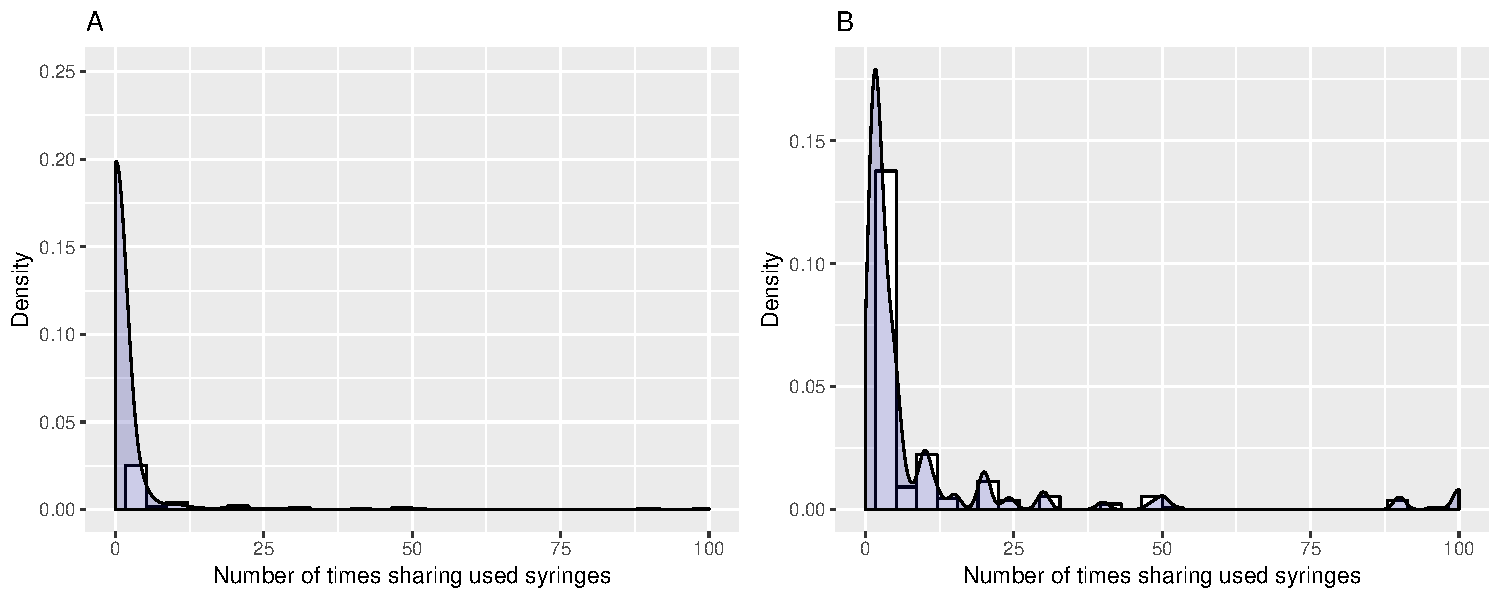
\includegraphics{Final_project_slides_files/figure-beamer/hist-1.pdf}

This shows us that the vast majority of participants (more than half)
reported zero for the outcome, which may cause problems for a poisson
model. It is also extremely right-skewed, also implying that a negative
binomial model may be a better fit.

\end{frame}

\begin{frame}{Compare models (2)}

\small
We also want to compare models with a few different tests, to see which
appears to have the best fit.

\begin{enumerate}
\def\labelenumi{\arabic{enumi}.}
\tightlist
\item
  Since the mixed models are nested, we can use a likelihood ratio test:
\end{enumerate}

\tiny

\begin{longtable}[]{@{}lll@{}}
\toprule
Model & Log Likelihood & P-value\tabularnewline
\midrule
\endhead
Poisson & -2231.753 &\tabularnewline
Neg Binom. & -1223.066 & 0\tabularnewline
\bottomrule
\end{longtable}

\vspace{-10pt} \small
~~~~~~ This tells us that the negative binomial model is significantly\\
\hspace*{0.333em}\hspace*{0.333em}\hspace*{0.333em}\hspace*{0.333em}\hspace*{0.333em}\hspace*{0.333em}
preferred over the poisson model.

\begin{enumerate}
\def\labelenumi{\arabic{enumi}.}
\setcounter{enumi}{1}
\tightlist
\item
  We can also compare the AIC of the mixed models, though this involves
  comparing likelihoods that ignore the repeated measures in our study:
\end{enumerate}

\vspace{-12pt} \tiny

\begin{longtable}[]{@{}ll@{}}
\toprule
Model & AIC\tabularnewline
\midrule
\endhead
Poisson & 4485.505\tabularnewline
Neg Binom. & 2470.133\tabularnewline
\bottomrule
\end{longtable}

\vspace{-10pt} \small
~~~~~~ This also suggests that the negative binomial model is a better
fit.\\
\textcolor{white}{.}

\end{frame}

\begin{frame}{Compare models (3)}

\small
We are concerned about strong violations of the assumption of no
informative censoring, for our GEE model. Yet we are also concerned
about overdispersion, as well as the large number of zeros in our
outcome, both of which may cause our poisson mixed methods model to be a
poor fit.

\vspace{12pt}

For these reasons, it is not surprising that the negative binomial model
may be the best fit.

\vspace{12pt}

We are not able to run comparison tests of fit for GEE compared to our
mixed models, so one of the best things to do is to look at our results,
including standard error.

\end{frame}

\begin{frame}{Results}

\tiny
 ~~~~~~~~~~~~~~~~~~~ ~~~~~~~~~~~~~~~~~~~~~~~~~~~~~~~~~~~~~~~~~~~GEE
~~~~~~~~~~~~~ ~~~~~~~~Mixed Model ~~~~~~~~~~~~~~Mixed Model\\
\hspace*{0.333em}\hspace*{0.333em}\hspace*{0.333em}\hspace*{0.333em}\hspace*{0.333em}\hspace*{0.333em}\hspace*{0.333em}\hspace*{0.333em}\hspace*{0.333em}\hspace*{0.333em}\hspace*{0.333em}\hspace*{0.333em}\hspace*{0.333em}\hspace*{0.333em}\hspace*{0.333em}\hspace*{0.333em}\hspace*{0.333em}\hspace*{0.333em}\hspace*{0.333em}\hspace*{0.333em}\hspace*{0.333em}\hspace*{0.333em}\hspace*{0.333em}\hspace*{0.333em}\hspace*{0.333em}\hspace*{0.333em}\hspace*{0.333em}\hspace*{0.333em}\hspace*{0.333em}\hspace*{0.333em}\hspace*{0.333em}\hspace*{0.333em}\hspace*{0.333em}\hspace*{0.333em}\hspace*{0.333em}\hspace*{0.333em}\hspace*{0.333em}\hspace*{0.333em}\hspace*{0.333em}\hspace*{0.333em}\hspace*{0.333em}\hspace*{0.333em}\hspace*{0.333em}\hspace*{0.333em}\hspace*{0.333em}\hspace*{0.333em}\hspace*{0.333em}\hspace*{0.333em}\hspace*{0.333em}\hspace*{0.333em}\hspace*{0.333em}\hspace*{0.333em}\hspace*{0.333em}\hspace*{0.333em}\hspace*{0.333em}\hspace*{0.333em}\hspace*{0.333em}\hspace*{0.333em}\hspace*{0.333em}\hspace*{0.333em}(Poisson)
~~~~~~~~~~ ~~~~~~~~~~~(Poisson) ~~~~~~~~~~~~~~~ (Neg Binom.)

\vspace{-8pt}

\begin{longtable}[]{@{}llllllllll@{}}
\toprule
Predictor & & Est. & p-value* & & Est. & p-value & & Est. &
p-value\tabularnewline
\midrule
\endhead
Never publicly inject & & ref & & & ref & & & ref &\tabularnewline
Occasionally/sometimes publicly inject & & 1.41 & 0.09 & & 2.44 &
1.9e-22 & & 3.28 & 0.00066\tabularnewline
Usually/Always publicly inject & & 2.28 & 0.01 & & 3.62 & 3.5e-39 & & 8
& 7.5e-08\tabularnewline
& & & & & & & & &\tabularnewline
Housed at study visit & & ref & & & ref & & & ref &\tabularnewline
Homeless at study visit & & -1.32 & 0.08 & & 1.24 & 0.05 & & 0.89 &
0.73\tabularnewline
& & & & & & & & &\tabularnewline
Male & & ref & & & ref & & & ref &\tabularnewline
Female & & -0.12 & 0.83 & & 0.96 & 0.91 & & 1.31 & 0.47\tabularnewline
Transgender & & -1.27 & 0.16 & & 1.01 & 0.99 & & 1.1 &
0.93\tabularnewline
& & & & & & & & &\tabularnewline
Age (year) & & -0.02 & 0.32 & & 0.96 & 0 & & 0.98 & 0.08\tabularnewline
& & & & & & & & &\tabularnewline
No stimulant use & & ref & & & ref & & & ref &\tabularnewline
Stimulant use & & 0.29 & 0.57 & & 0.65 & 2.4e-05 & & 1.87 &
0.03\tabularnewline
& & & & & & & & &\tabularnewline
No opiate use & & ref & & & ref & & & ref &\tabularnewline
Opiate use & & -0.2 & 0.73 & & 0.74 & 0.0031 & & 1.74 &
0.09\tabularnewline
& & & & & & & & &\tabularnewline
No binge drinking & & ref & & & ref & & & ref &\tabularnewline
Binge drinking & & -0.33 & 0.45 & & 0.88 & 0.041 & & 1.59 &
0.05\tabularnewline
\bottomrule
\end{longtable}

\vspace{-14pt} ~~~~~~*p-values based on robust SEs

\footnotesize
We can see from these results that the inference is similar across
models, though the magnitude of the effect is much stronger in the
negative binomial model, and the standard error is much larger for the
GEE model.

\end{frame}

\begin{frame}[fragile]{Attempt a compelling graph related to your
research question}

\%\%\%\%\%\%\%\%\%\%\%\%\%\%\%\\
MAKE THE GRAPH - Lizzy\\
\%\%\%\%\%\%\%\%\%\%\%\%\%\%\%

\begin{Shaded}
\begin{Highlighting}[]
\CommentTok{#library(ggplot2)}
\CommentTok{#library(lme4)}

\CommentTok{#"lme4:::getNBdisp(modelnb_categorical)" gets theta from NB model}
\CommentTok{#error: Fitting failed for 978 group(s), probably because a factor only had one level: contrasts can be applied only to factors with 2 or more levels}

\CommentTok{#fits <- lmList(TIMESHARE ~ PUBINJ_3cat + HOMELESS + GENDER + AGE + factor(ANYSTIM) + factor(ANYOPIATE) + factor(binge) | SUBJECT, family = negative.binomial(0.4647), data = dfslong, na.action = na.omit)}


\NormalTok{##################}
\CommentTok{#trying alternative method using predict function}

\CommentTok{#model_p <-predict(modelnb_categorical)}
\CommentTok{#model_p <- as.data.frame(model_p)}

\CommentTok{#Error in data.frame(dfslong$SUBJECT, dfslong$PUBINJ_3cat, model_p) : arguments imply differing number of rows: 2934, 1069}
\CommentTok{#predicted_df <- data.frame(dfslong$SUBJECT, dfslong$PUBINJ_3cat, model_p)}
\CommentTok{#colnames(predicted_df) <- c("subject", "pubinj", "predicted_y")}

\CommentTok{# modify this code if i can get it to work}
\CommentTok{#gg_nb <- ggplot(data = predicted_df, aes(x = time, y = predicted_y, group=id)) +}
  \CommentTok{#geom_line(aes(color=factor(id))) + theme_classic() +}
  \CommentTok{#ggtitle("Strength over Time, Predicted for Each Individual") +}
  \CommentTok{#labs(y= "Lin Mod Prediction of CD4 ", x = "Time") +}
  \CommentTok{#facet_grid(. ~ drug.base) +}
  \CommentTok{#theme(legend.position="none")}
\end{Highlighting}
\end{Shaded}

\end{frame}

\begin{frame}{Discussion}

Interpret your results both with regard to the substantive question of
interest as well as any statistical issues.

In multivariable analysis across all timepoints, participants who
usually/always injected publicly had 7.99 (p \textless{} .001) times
higher counts of receptive syringe sharing over the past six months,
compared to those who never publicly injected, controlling for age,
gender, homelessness, stimulant injecting, opioid injecting, and binge
drinking. Participants who occasionally/sometimes injected publicly had
3.28 (p \textless{} .001) times higher counts of receptive syringe
sharing over the past six months, compared to those who never publicly
injected, controlling for covariates.

\underline{Conclusion}: Injecting publicly is associated with receptive
syringe sharing among PWID, with higher frequency of public injection
corresponding to higher frequency of sharing syringes. This suggests
that PWID may be rushing their injections in public settings by using
shared syringes. Findings underscore the need for safer environment
interventions, such as supervised consumption sites, where PWID can take
their time and use sterile injecting equipment.

\underline{Limitations}: This study had significant loss-to-follow-up.
The authors used complete case analysis for the sake of simplicity,
however results may change if other missing data approaches were
applied, such as inverse probability of censoring weighting or multiple
imputation.

\end{frame}

\end{document}
